\documentclass[11pt]{article}
\usepackage{amsmath}
\usepackage{amssymb}
\usepackage{graphicx}
\usepackage{fancyhdr}
\usepackage{enumerate}
\usepackage{float}
\usepackage{graphicx}
\usepackage{titlesec}
\usepackage[colorlinks=true,urlcolor=blue]{hyperref}

\titlespacing{\subsubsection}{0pt}{0pt}{0pt}

% No page numbers
%\pagenumbering{gobble}

% INFORMATION SHEET (DO NOT EDIT THIS PART) ---------------------------------------------
\newcommand{\addinformationsheet}{
\clearpage
\thispagestyle{empty}
\begin{center}
\LARGE{\bf \textsf{Information sheet\\CS246: Mining Massive Data Sets}} \\*[4ex]
\end{center}
\vfill
\textbf{Assignment Submission } Fill in and include this information sheet with each of your assignments.  This page should be the last page of your submission.  Assignments are due at 11:59pm and are always due on a Thursday.  All students (SCPD and non-SCPD) must submit their homework via Gradescope (\url{http://www.gradescope.com}). Students can typeset or scan their homework. Make sure that you answer each (sub-)question on a separate page. That is, one answer per page regardless of the answer length. Students also need to upload their code on Gradescope. Put all the code for a single question into a single file and upload it.  
\\
\\
\textbf{Late Homework Policy } Each student will have a total of {\em two} late periods. {\em Homework are due on Thursdays at 11:59pm PT and one late period expires on the following Monday at 11:59pm PT}.  Only one late period may be used for an assignment.  Any homework received after 11:59pm PT on the Monday following the homework due date will receive no credit.  Once these late periods are exhausted, any assignments turned in late will receive no credit.
\\
\\
\textbf{Honor Code } We strongly encourage students to form study groups. Students may discuss and work on homework problems in groups. However, each student must write down their solutions independently, i.e., each student must understand the solution well enough in order to reconstruct it by him/herself.  Students should clearly mention the names of all the other students who were part of their discussion group. Using code or solutions obtained from the web (GitHub/Google/previous year's solutions etc.) is considered an honor code violation. We check all the submissions for plagiarism. We take the honor code very seriously and expect students to do the same. 
\vfill
}

% MARGINS (DO NOT EDIT) ---------------------------------------------
\oddsidemargin  0.25in \evensidemargin 0.25in \topmargin -0.5in
\headheight 0in \headsep 0.1in
\textwidth  6.5in \textheight 9in
\parskip 1.25ex  \parindent 0ex \footskip 20pt
% ---------------------------------------------------------------------------------

% HEADER (DO NOT EDIT) -----------------------------------------------
\newcommand{\problemnumber}{0}
\newcommand{\myname}{name}
\newfont{\myfont}{cmssbx10 scaled 1000}
\pagestyle{fancy}
\fancyhead{}
\fancyhead[L]{\myfont Question \problemnumber, Homework 4, CS246}
%\fancyhead[R]{\bssnine \myname}
\newcommand{\newquestion}[1]{
\clearpage % page break and flush floats
\renewcommand{\problemnumber}{#1} % set problem number for header
\phantom{}  % Put something on the page so it shows
}
% ---------------------------------------------------------------------------------


% BEGIN HOMEWORK HERE
\begin{document}

% Question 1(a)
\newquestion{1(a)}

In the beggining all nodes have initial feature vector $x = [1]$. 
In each iteration this vector is updated to the sum of node's current embedding and embeddings of it's neighbors.
Lets write the embedding of each node next to it in the picture.

\begin{figure}[H]
    \centering
    Graph 1: \\
    \includegraphics[width=0.2\textwidth]{pictures_q1/1_1.png}  
    \includegraphics[width=0.05\textwidth]{pictures_q1/empty.png}   
    \includegraphics[width=0.2\textwidth]{pictures_q1/2_1.png}     
    \includegraphics[width=0.05\textwidth]{pictures_q1/empty.png}   
    \includegraphics[width=0.2\textwidth]{pictures_q1/3_1.png}     
    \includegraphics[width=0.05\textwidth]{pictures_q1/empty.png}   
    \includegraphics[width=0.2\textwidth]{pictures_q1/4_1.png} 
    \\
    Graph 2: \\
    \includegraphics[width=0.2\textwidth]{pictures_q1/1_2.png}  
    \includegraphics[width=0.05\textwidth]{pictures_q1/empty.png}   
    \includegraphics[width=0.2\textwidth]{pictures_q1/2_2.png}  
    \includegraphics[width=0.05\textwidth]{pictures_q1/empty.png}   
    \includegraphics[width=0.2\textwidth]{pictures_q1/3_2.png}  
    \includegraphics[width=0.05\textwidth]{pictures_q1/empty.png}   
    \includegraphics[width=0.2\textwidth]{pictures_q1/4_2.png}
\end{figure}

We can see that the embeddings for the red nodes in the given graphs begin to 
differ after three hidden layers. On graph $1$ the embedding
on 3rd layer of the red node is $[18]$ and on graph $2$ it is $[17]$.

% Question 1(b)
\newquestion{1(b)}

To reduce Janossy pooling to mean aggregation, we need to define a function $\rho_\phi$
such that it computes the mean of the embeddings of the neighbouring nodes of the sequence. 

This can be expressed as 
$$ \rho_\phi (h_{u_1}^{k-1}, h_{u_2}^{k-1}, \dots h_{u_{|N(v)|}}^{k-1})_ {\pi} = \frac{1}{| N(v) |} \sum_{u \in N(v)} h_u^{k-1} , $$

here $h_u^{k-1}$ represents the embedding of neighbour node $u$ of $v$ at 
layer $k-1$ and $N(v)$ represents the neighbourhood of node $v$.
Observe that the right side is not depended on permutation $\pi$, therefore the aggregation
function which is the average over all permutations from $\Pi$ can be rewriten as:
\begin{align*}
    \text{aggregate}_\text{janossy} \left( \left\{ h_u^{k-1} , \forall u \in N(v) \right\} \right) &= \frac{1}{| \Pi |} \sum_{\pi \in \Pi}\rho_\phi (h_{u_1}^{k-1}, h_{u_2}^{k-1}, \dots h_{u_{|N(v)|}}^{k-1})_ {\pi} \\
    &= \frac{1}{| \Pi |} \sum_{\pi \in \Pi} \frac{1}{| N(v) |} \sum_{u \in N(v)} h_u^{k-1} \\
    &= \frac{1}{| \Pi |} | \Pi | \frac{1}{| N(v) |} \sum_{u \in N(v)} h_u^{k-1} \\
    &= \frac{1}{| N(v) |} \sum_{u \in N(v)} h_u^{k-1}
\end{align*}

By defining $\rho_\phi$ in this way, Janossy pooling reduces to mean aggregation, as 
it computes the mean of the embeddings of all neighbor nodes for each permutation of 
the input sequence. This aligns with the concept of mean aggregation where information 
from all neighbors is aggregated by taking the mean of their embeddings.

Janossy pooling is potentially more expressive than mean pooling. This is because 
Janossy pooling considers all permutations of neighbor embeddings and applies a 
function (such as an LSTM) to each permutation, whereas mean pooling simply 
computes the average of neighbor embeddings without considering permutations.
We also observed this in our example, since we were able to reduce janossy pooling to 
mean aggregation function.

% Question 1 (c)
\newquestion{1(c)}

Now we consider breadth-first search, where at every step, nodes that are connected 
to already visited nodes become visited. Message function of this approach is 
\[ M (h_v^k) = h_v^k 
    \text{.}
\]
Here the message function returns $1$ if the node $v$ was already visited, otherwise it returns $0$.

The aggregation function collects messages from all neighboring nodes. We can use the sum of 
all neighbouring nodes, by which we achive that update function works properly. Define 
aggregation function as:
$$ h_{N(v)}^{k+1} = \sum_{u \in N(v)} h_u^k \text{.}$$

With the update function we would like to update the node's representation.
Since BFS works in a binary manner (visited or not visited), the update function should set the 
representation of $v$ to either $0$ or $1$. It should become $1$ if one of the neighboring nodes is 
$1$. That is exactly when an aggregation function is greater than zero:
$$ h_v^{k+1} = \left\{
    \begin{array}{lr}
        1, & h_{N(v)}^{k+1} > 0 \\
        0, & \text{otherwise}
    \end{array}
\right\} \text{.}
$$

For the aggregation function we could also use logical OR operator. If one of the neighbouring nodes
of $v$ is $1$, than $h_v$ should be $1$ in the next iteration:
$$ h_{N(v)}^{k+1} = OR(h_{N(v)}^k) \text{.}$$
If we defined aggregation function like this, the update function is identical to aggregation function: 
$$ h_v^{k+1} = h_{N(v)}^{k+1} \text. $$

% Question 2(a)
\newquestion{2(a)}

When calculating the gain function for wine, we devide all $100$ people on those who like wine and those who do not.
This way we get two groups of $50$ people. Then we further devide each of the two groups on those who like beer and 
those who do not. In both groups there are $20$ people who like beer and $30$ who do not.
% We can understand this devisions from a sketch:  mogoče
Therefore value of gain function $G$ for wine is $2.0$, calculated from
\begin{align*}
    G_{wine} &= I(D) - ( I(D_L) + I(D_R)) = \\
    &= \left( 100 \times \left( 1 - \left( \frac{50}{100} \right)^2 - \left(\frac{50}{100}\right)^2 \right)\right) - \\
    & - \left( 50 \times \left(1 - \left( \frac{20}{50} \right)^2 - \left(\frac{30}{50}\right)^2 \right) \right) - \\
    & - \left( 50 \times \left(1 - \left( \frac{20}{50} \right)^2 - \left(\frac{30}{50}\right)^2 \right) \right) = \\
    &= 50.0 - 24.0 - 24.0 =\\
    &= 2.0
\end{align*}

When caluclating the gain function for running, we first form two groups, a group of $30$ people who like running
and a group of $70$ who do not. Then we devide a group of $30$ who like running to $20$ who also like beer and $10$
that do not. Similarly we devide the group of $70$ to $20$ who like beer, the remaining $50$ do not. Gain function for 
running is calculated as follows:
\begin{align*}
    G_{running} &= I(D) - ( I(D_L) + I(D_R)) = \\
    &= \left( 100 \times \left( 1 - \left( \frac{30}{100} \right)^2 - \left(\frac{70}{100}\right)^2 \right)\right) - \\
    & - \left( 30 \times \left(1 - \left( \frac{20}{30} \right)^2 - \left(\frac{10}{30}\right)^2 \right) \right) - \\
    & - \left( 70 \times \left(1 - \left( \frac{20}{70} \right)^2 - \left(\frac{50}{70}\right)^2 \right) \right) = \\
    &= 42.0 - 13.333 - 28.571 =\\
    &= 0.095
    \text{.}
\end{align*}

We do the same for pizza. First form two groups of people - $80$ who like pizza and $20$ who dislike it.
Then devide the first group on $30$ who like beer and $50$ who do not, and the second group on $10$ who like 
beer and $10$ who do not. Calculating the gain function we obtain:
\begin{align*}
    G_{pizza} &= I(D) - ( I(D_L) + I(D_R)) = \\
    &= 32.0 - 37.5 - 10.0 = \\
    &= - 15.5
    \text{.}
\end{align*}

We see that gain is maximal for wine. Therefore if we were to maximize
the gain $G$ using the gini index metric, we should use wine attribute 
to split the data at root.

% Question 2(b)
\newquestion{2(b)}

Since attribute $a_1$ has the most significant dependance on target $y$, the root node of 
the decision tree should be assosiated with $a_1$. This will lead to two child nodes, $a_1 = 0$ 
and $a_1 = 1$. Other attributes may contribute to splitting decisions, but their impact will 
be smaller than of $a_1$.

Because we are building a complete binary tree, we use values of all attributes.
Since there are $100$ attributes in total and each level of the tree represents a 
decision based on one of these attributes, the height of the tree, 
which corresponds to the number of levels, will be equal to the number of 
attributes. 

The desired decision tree should also split on $a_1$ at the root node, since it is the most
informative. This way it will return the correct answer with $99\%$ probability. 
% After the split, left and right subtrees have the same number of elements ($ 2^{99}$ ), therefore further splits will act the same on both subtrees.
Splitting the tree further by 
other attributes would only lower this probability, since 
the answer is returned by the leaf node and the leaf node has the probability of returning the 
correct answer lower then $99\%$.



% It can also consider some other attributes, to improve predictability.
% But to avoid overfitting, it should not consider all $100$ attributes. We could restrict it 
% to a predetermined depth. 
% 
% If we are able to compare importance of attributes $a_2 \dots a_{100}$, we should use 
% those of the highest importance following $a_1$, until reaching desired depth. By 
% prioritizing informative attributes and generalizing effectively, the desired decision 
% tree will achieve better generalization performance on unseen data, thus avoiding overfitting. 
% This approach ensures that the model captures meaningful patterns in the data while preventing 
% it from memorizing noise or irrelevant details.

% Question 3(a)
\newquestion{3(a)}

Lets prove
$$ \text{cost} (S, T) \leq 2 \sum_{i=1}^{l} \text{cost} (S_i, T_i) + 2 \cdot \text{cost}_{\omega} (\hat{S}, T)\text{.} $$

For every node $x \in S$ we use triangular inequality:
$$ d(x, T) \leq d(x, t_{ij}) + d (t_{ij}, T)\text{,} $$
where $t_{ij} \in T_i \subset \hat{S} $ is the centroid nearest to $x$, 
meaning $x \in S_i$ for some $i$. $T$ is defined as in the algorithm.

We can square this inequality, obtaining
$$ d(x, T)^2 \leq \left( d(x, t_{ij}) + d (t_{ij}, T) \right)^2 \leq 2 d(x, t_{ij})^2 + 2 d (t_{ij}, T)^2 \text{,} $$
where in the second inequality we used a fact given in instructions: $(a + b)^2 \leq 2a^2 + 2b^2$.

Because this inequality holds true for every node $x \in S$, it must also hold true
for the sum over all $x \in S$, by which we get 
\begin{equation}
    \label{eq3a}
    \sum_{x \in S} d(x, T)^2 \leq 2 \sum_{i=1}^{l} \sum_{x \in S_i} d(x, t_{ij})^2 + 2 \sum_{t_{ij} \in \hat{S}} \omega (t_{ij}) d (t_{ij}, T)^2 \text{.}
\end{equation}

Lets see that in all three summands we summed over all $x \in S$. To see this in summand on the left is trivial. 
In the second summand, we sum over all $x \in S_1 \dots x \in S_l$, meaning we sum over all $x \in S_1 \cup \dots \cup S_l = S$. 
Here $t_{ij} \in T_i$ is the nearest centroid from $x \in S_i$, defined in the sum.
In the third sum, we are summing over all centroids in $\hat{S} = \bigcup_{i=1}^{l} T_i$.
Here we count each distance from $t_{ij}$ to $T$ as many times as there are nodes that are nearest to centroid $t_{ij}$.
This is exactly the definition of $\omega (t_{ij})$.

We know that distance from a point to a set of points is the minimum distance from a given point to each point in the set.
Since $t_{ij}$ is defined as a centroid from $T_i$ nearest to $x$, we can rewrite $d(x, t_{ij}) = d(x, T_i)$.

From the definition of cost function we see
\begin{align*}
    \sum_{x \in S} d(x, T)^2 &= \text{cost} (S, T) \text{,}\\
    \sum_{x \in S_i} d(x, T_i)^2 &= \text{cost} (S_i, T_i) \text{,}\\
    \sum_{t_{ij} \in \hat{S}} \omega (t_{ij}) d (t_{ij}, T)^2 &= \text{cost} (\hat{S}, T) \text{.}  
\end{align*}

Now lets rewrite equation \eqref{eq3a}. We get the final result
$$ \text{cost} (S, T) \leq 2 \sum_{i=1}^{l} \text{cost} (S_i, T_i) + 2 \cdot \text{cost}_{\omega} (\hat{S}, T)\text{.} $$

% Question 3(b)
\newquestion{3(b)}

Lets prove
$$ \sum_{i=1}^{l} \text{cost} (S_i, T_i) \leq \alpha \cdot \text{cost} (S, T^*) \text{.}$$

Because we assume we have an algorithm ALG which is
an $\alpha$-approximate k-means clustering algorithm, we know 
$$ \text{cost} (S_i, T_i) \leq \alpha \min_{ |T'|=k} \left\{ \text{cost} (S_i, T') \right\} \text{.} $$

Since we take a subset $S_i \subset S$ and a fixed set of centroids $T^*$, we can bound
$$ \min_{ |T'|=k} \left\{ \text{cost} (S_i, T') \right\} \leq \text{cost} (S_i, T^*) \text{.} $$

Lets bound the left side of inequality we are proving 
\begin{align*}
    \sum_{i=1}^{l} \text{cost} (S_i, T_i) &\leq \alpha \sum_{i=1}^{l} \text{cost} (S_i, T^*) \\
    &= \alpha \sum_{i=1}^{l} \sum_{x \in S_i} d (x, T^*) \\
    &= \alpha \sum_{x \in S} d (x, T^*) \\
    &= \alpha \cdot \text{cost} (S, T^*)
\end{align*}

In third line we used that $S = S_1 \cup \dots \cup S_l$ is a disjunct union.

% Question 3(c)
\newquestion{3(c)}

First lets prove 
\begin{equation}
    \label{eq2c_1}
    \text{cost}_{\omega} \left( \hat{S} , T \right) \leq \alpha \cdot \text{cost}_{\omega} \left( \hat{S} , T^* \right) \text{.}
\end{equation}
Since we use algorithm ALG on $\hat{S}$ to find $T$, from the definition of ALG we know
    $$ \text{cost}_{\omega} \left( \hat{S} , T \right) \leq \alpha \min_{|T'| = k} \left\{ \text{cost}_{\omega} \left( \hat{S} , T' \right) \right\} $$
Since $T^*$ is fixed set of cardinality $k$, we know that its cost is at least the minimum cost over all sets of cardinality $k$.
Mathematically this can be written as
    $$ \min_{|T'| = k} \left\{ \text{cost}_{\omega} \left( \hat{S} , T' \right) \right\} \leq \text{cost}_{\omega} (\hat{S}, T^*) \text{.}$$
This proves the first inequality.

Now we would like to prove 
\begin{equation}
    \label{eq3c_2}
    \text{cost}_{\omega} (\hat{S}, T^*) \leq 2 \sum_{i = 1}^{l} \text{cost} (S_i, T_i) + 2 \cdot \text{cost} (S, T^*) \text{.}
\end{equation}
For every $x \in S$ we can use triangular ineguality
    $$ d \left( t_{ij}, T^* \right) \leq d \left( x, t_{ij} \right) + d \left( x, T^* \right) \text{,}$$
where $t_{ij}$ is centroid nearest to $x$.
% This can be observed from a simple sketch:
Squaring the whole inequality gives
    $$ d \left( t_{ij}, T^* \right)^2 \leq \left( d \left( x, t_{ij} \right) + d \left( x, T^* \right) \right)^2 \leq 2 d \left( x, t_{ij} \right)^2 + 2 d \left( x, T^* \right)^2 \text{.}$$
Since $t_{ij} \in T_i$ is the nearest to $x$ from all point in $T_i$, we know $d \left( x, t_{ij} \right) = d \left( x, T_i \right)$ from the definition of Euclidean distance between a point and a set.
Now summing over all $x \in S$ we obtain
    $$ \sum_{t_{ij} \in T_i} \omega (t_{ij}) d \left( t_{ij}, T^* \right)^2 \leq 2 \sum_{i = 1}^{l} \sum_{x \in S_i} d \left( x, T_i \right)^2 + 2 \sum_{x \in S} d \left( x, T^* \right)^2 \text{.} $$
When summing over all $x \in S$ we count every distance $ d \left( t_{ij}, T^* \right)^2 $ as many times as there are points $x \in S$ that are 
nearest to $t_{ij}$, thus we muliply with $\omega (t_{ij})$. 
Now using the definition of cost function we obtain
    $$ \text{cost}_{\omega} (\hat{S}, T^*) \leq 2 \sum_{i = 1}^{l} \text{cost} (S_i, T_i) + 2 \cdot \text{cost} (S, T^*) \text{.} $$


With the above proofs the final result is just a simple calculation:
\begin{align}
    \text{cost} \left( S, T \right) &\leq 2 \cdot \text{cost}_{\omega} (\hat{S}, T) + 2 \sum_{i=1}^{l} \text{cost} (S_i, T_i)\label{4} \\
    &\leq 2 \alpha \cdot \text{cost}_{\omega} \left( \hat{S} , T^* \right) + 2 \sum_{i=1}^{l} \text{cost} (S_i, T_i) \label{5} \\
    &\leq 2 \alpha \cdot \text{cost}_{\omega} \left( \hat{S} , T^* \right) + 2 \alpha \cdot \text{cost} (S, T^*) \label{6} \\
    &\leq 2 \alpha \left( 2 \sum_{i = 1}^{l} \text{cost} (S_i, T_i) + 2 \cdot \text{cost} (S, T^*) \right) + 2 \alpha \cdot \text{cost} (S, T^*) \label{7} \\
    &\leq 2 \alpha \left( 2 \alpha \cdot \text{cost} (S, T^*) + 2 \cdot \text{cost} (S, T^*)\right) + 2 \alpha \cdot \text{cost} (S, T^*) \label{8} \\
    &\leq \left( 4 \alpha^2 + 6 \alpha \right) \cdot \text{cost} (S, T^*) \label{9} \text{,}
\end{align}

where we utilized part 3(a) to address inequality (4). Then, in \eqref{5}, we referenced equation \eqref{eq2c_1}, 
followed by employing part 3(b) in \eqref{6}. Inequality \eqref{7} relied on \eqref{eq3c_2}. In \eqref{8}, 
we once more employed part 3(b), and finally, in \eqref{9}, we utilized basic multiplication and summation 
to derive the final result.

% Question 4(a)
\newquestion{4(a)}

In this question we would like to prove
\begin{equation}
    \label{eq4a}
    \Pr \left[ \tilde{F} [i] \leq F [i] + \epsilon t \right] \geq 1 - \delta \text{.}
\end{equation}

Rewrite this inequality as
\begin{align*}
    1 - \Pr \left[ \tilde{F} [i] \geq F [i] + \epsilon t \right] &\geq 1 - \delta  \text{,}\\
    \Pr \left[ \tilde{F} [i] \geq F [i] + \epsilon t \right] &\leq \delta \text{.}
%    \Pr \left[ \tilde{F} [i] - F [i] \geq \epsilon t \right] &\leq \delta \text{.}
\end{align*}
Therefore proving \eqref{eq4a} is equal to proving the last inequality above.
% We can use Markov inequality on the left side of the last inequality, since both $\tilde{F} [i] - F [i] \geq 0$ and $\epsilon t \geq 0$:
%     $$ \Pr \left[ \tilde{F} [i] - F [i] \geq \epsilon t \right] \leq \frac{\mathbb{E} [ \tilde{F} [i] - F [i] ] }{\epsilon t} \text{.}$$
% Now using linearity of expected value we get
%     $$ \frac{\mathbb{E} [ \tilde{F} [i] - F [i] ] }{\epsilon t} \leq \frac{\mathbb{E} [ \tilde{F} [i] ] - \mathbb{E} \left[ F [i] \right] }{\epsilon t} \text{.}$$
% From properties given in instructions we know that 
%     $$ \mathbb{E} \left[ c_{j, h_j (i)} \right] \leq F [i] - \frac{\epsilon}{e} \left( t - F[i] \right) $$
% for every $1 \leq i \leq n$ and every $1\leq j \leq \lceil \log \left( \frac{1}{\delta} \right) \rceil $. Therefore this property holds 
% also for $\tilde{F} [i] = \min_j \{  c_{j, h_j (i)} \}$. We also know that $F[i]$ is constant and that expected value of a constant is constant
% itself. We obtain
%     $$ \frac{\mathbb{E} [ \tilde{F} [i] ] - \mathbb{E} \left[ F [i] \right] }{\epsilon t} = \frac{F [i] - \frac{\epsilon}{e} \left( t - F[i] \right) - F[i]}{\epsilon t} = \frac{t - F[i]}{e t} = \frac{1}{e} \left( 1 - \frac{F[i]}{t} \right) \text{.}$$
% 
% If we prove $\frac{1}{e} \left( 1 - \frac{F[i]}{t} \right) \leq \delta$, we prove \eqref{eq4a}, therefore lets rewrite it as 
% \begin{align}
%     1 - \frac{F [i]}{t} \leq e \delta \text{,} \nonumber \\
%     \frac{F [i]}{t} \geq 1 - e \delta \text{.} \label{eq4a1}
% \end{align}
% $F [i]$ is defined as the number of times $i$ appeared in the data stram $S$, therefore it is bounded by $0 \leq F[i] \leq t$.
% Dividing this inequality with $t$ we get $0 \leq \frac{F[i]}{t} \leq 1$. Combining we get
% \begin{align*}
%     1 - e \delta &\leq 1 \\
%     e \delta \geq 0 \text{,}
% \end{align*}
% which is true, since $e \geq 0$ and $\delta > 0$. Because this is true, inequality \eqref{eq4a1} also holds, proving \eqref{eq4a}.

Lets rewrite the left side. First we use the definition of $\tilde{F} [i]$.
\begin{align*}
    \Pr \left[ \tilde{F} [i] \geq F [i] + \epsilon t \right] &= \Pr \left[ \min \{ c_{j, h_j (i)} \} > F [i] + \epsilon t \right]
    \intertext{Since all $c_{j, h_j (i)}$ are greater then their minimum, this probability is equal to the following.} 
    &= \Pr \left[ \bigwedge_{j=1}^{\lceil \log \frac{1}{\delta} \rceil} \left( c_{j, h_j (i)} > F [i] + \epsilon t \right)\right] 
    \intertext{Because all expressions in the conjunction are independent, we can rewrite the latest probability as a product.}
    &= \prod_{j=1}^{\lceil \log \frac{1}{\delta} \rceil} \Pr \left[ c_{j, h_j (i)} > F [i] + \epsilon t \right] = \prod_{j=1}^{\lceil \log \frac{1}{\delta} \rceil} \Pr \left[ c_{j, h_j (i)} - F [i] > \epsilon t \right]
    \intertext{Now we can use Markov inequality on each factor, since both sides are positive. This follows from $F [i] \leq \tilde{F} [i] \leq c_{j, h_j(i)}$ for every $j$ and $i$. }
    &\leq \prod_{j=1}^{\lceil \log \frac{1}{\delta} \rceil} \frac{\mathbb{E} [c_{j, h_j (i)} - F [i]]}{\epsilon t}
    = \prod_{j=1}^{\lceil \log \frac{1}{\delta} \rceil} \frac{\mathbb{E} [c_{j, h_j (i)}] - F [i]}{\epsilon t}
    \intertext{From instructions we know that for any $1 \leq i \leq n$ and $1 \leq j \leq \lceil \log \frac{1}{\delta} \rceil$ it holds $\mathbb{E} [c_{j, h_j (i)}] \leq F [i] + \frac{\epsilon}{e} \left( t - F[i] \right)$, therefore we can bound the last expression with}
    &\leq \prod_{j=1}^{\lceil \log \frac{1}{\delta} \rceil} \frac{F [i] + \frac{\epsilon}{e} \left( t - F[i] \right) - F [i]}{\epsilon t} = 
    \prod_{j=1}^{\lceil \log \frac{1}{\delta} \rceil} \frac{\left( t - F[i] \right)}{e t}
    \intertext{We see that the above expression is not dependent on $j$, therefore it is equal to}
    &= \left( \frac{\left( t - F[i] \right)}{e t} \right)^{\lceil \log \frac{1}{\delta} \rceil}
%    &\leq \Pr \left[ \tilde{F} [i] > F [i] + \epsilon t \right]^{\lceil \log \frac{1}{\delta} \rceil} = \Pr \left[ \tilde{F} [i] - F [i] > \epsilon t \right]^{\lceil \log \frac{1}{\delta} \rceil} \\
%    \intertext{Both sides of the inequality in the probability function are greater than zero, which is given in the instructions, therefore we can use Markov bound.}
%    &\leq \left( \frac{\mathbb{E} [ \tilde{F} [i] - F [i] ] }{\epsilon t} \right)^{\log \frac{1}{\delta}} \\
%    \intertext{Now using the bound on $\tilde{F} [i]$ given in instructions and the fact that $F [i]$ is a constant, we obtain}
%    &\leq \left( \frac{F [i] + \frac{\epsilon}{e} \left( t - F[i] \right) - F [i]}{\epsilon t} \right)^{\log \frac{1}{\delta}} \\
%    &= \left( \frac{\frac{\epsilon}{e} \left( t - F[i] \right) }{\epsilon t} \right)^{\log \frac{1}{\delta}} \\
    = \left( \frac{1}{e} \left( 1 - \frac{F [i]}{t} \right) \right)^{\log \frac{1}{\delta}} \\
    \intertext{$F [i]$ is defined as the number of times $i$ appeared in the data stram $S$, therefore it is bounded by $0 \leq F[i] \leq t$. Dividing this inequality with $t$ we get $0 \leq \frac{F[i]}{t} \leq 1$.}
    &\leq \left( \frac{1}{e} \right)^{\log \frac{1}{\delta}} = e^{\log \delta} = \delta
\end{align*}

% Question 4(b)
\newquestion{4(b)}

\begin{figure}[H]
    \centering
    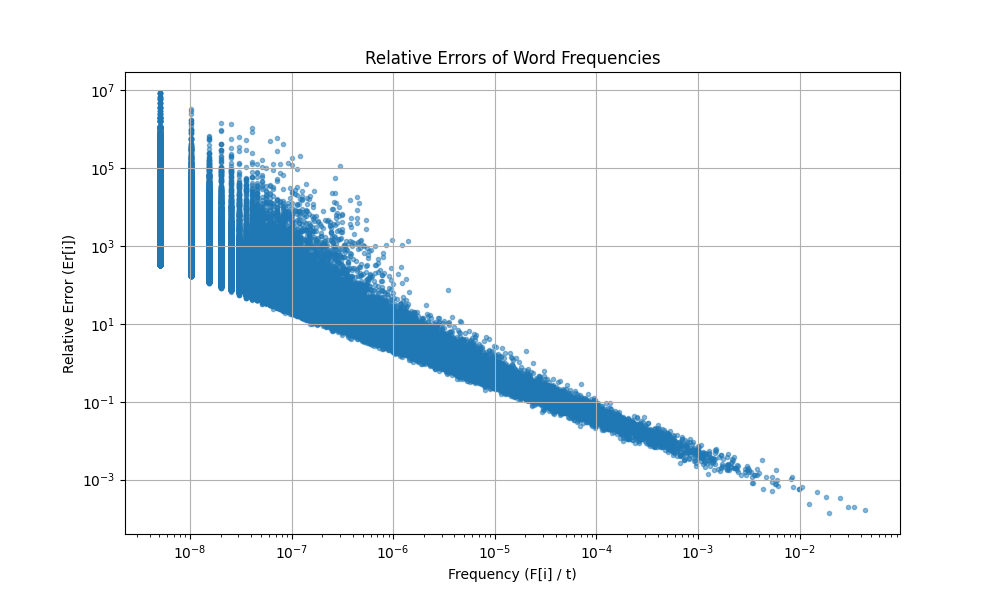
\includegraphics[width=\textwidth]{q4/plot.png} 
    \caption{The plot of relative errors depending on word frequency.}
\end{figure}

What is an approximate condition on a word frequency in the document to have a relative error below $1 = 10^0$ ?

The frequency of such words should be approximately higher than $10^{-5}$.

% Information sheet
% Fill out the information below (this should be the last page of your assignment)
\addinformationsheet
\vfill

{\Large
\textbf{Your name:} Lucija Fekonja  % Put your name here
\\
\\
\textbf{Email:} lf90992@student.uni-lj.si{\hspace*{3cm}}  % Put your e-mail here
\textbf{SUID:} 27232071   % Put your student ID here
\\*[2ex] 
}
Discussion Group: Nik Mrhar   % List your study group here
\\
\vfill\vfill
I acknowledge and accept the Honor Code.\\*[3ex]
\bigskip
\textit{(Signed)} 
LF  % Replace this line with your initials
\vfill






\end{document}